%----------------------------------------------------------------------------
\chapter{Sequential modeling}

This chapter focuses on the theoretical background of processing sequential data. As relatively simple deep learning-based solutions are surprisingly good with sequential data, I concentrate on neural network-based approaches.

Sequential modeling is a powerful way to solve numerous tasks, like video processing, time series prediction, or natural language processing. Many tasks can be modeled sequentially. The key is to project the domain problem to the proper abstraction. The categorization is partly based on source \cite{SequentialLecture}. There are different types of sequential tasks:

\begin{itemize}
  \item Vanilla approach processes the input in a \textit{single-input-single-output} (SISO) manner: for example, one frame of a video is classified independently of others. This is the case when the model has a single input image and makes classification.
  \item In a \textit{single-input-multiple-output} (SIMO) model, there is a single input and multiple possible outputs. For example, when an image contains multiple characters, the input is a single image, and the output is the sequence of characters in it.
  \item \textit{multiple-input-single-output} (MISO) models receive multiple inputs and output a single prediction. For example, the inputs are words of a textual review, and the prediction is the writer's sentiment.
  \item \textit{multiple-input-multiple-output} (MIMO) models receive multiple inputs and predict multiple outputs. These approaches can be divided into further subcategories:
    \begin{itemize}
        \item Some models receive multiple inputs and immediately output the prediction based on that. In video classification, a model usually receives multiple frames and outputs the class for each time frame, but these are predicted simultaneously, depending on each other.
	   \item In another configuration, popular in machine translation, models receive an input text and predict the current translated text on the fly, based on the current input. Here, input- and output sequences are shifted relative to each other (some input characters are needed for the first prediction). For example, Google Translate is a model of this kind.
    \end{itemize}
\end{itemize}

A summary of the different tasks is illustrated by Figure \ref{fig:task_types}.

\begin{figure}[htb]
 \centerline{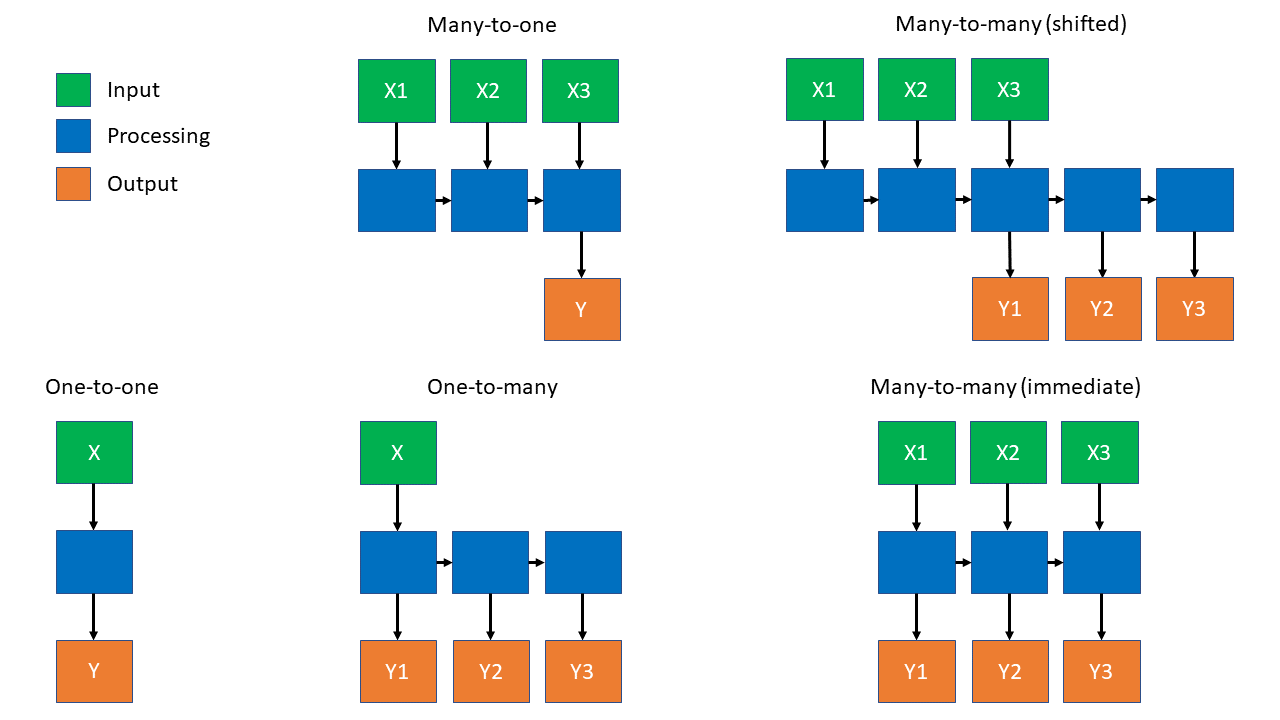
\includegraphics[width=1.0\columnwidth]{.//Figure/Sequential/task_types.png}}
 \caption{The different types of sequential tasks.}
 \label{fig:task_types}
\end{figure}

Sequential data can be processed with different network types. In the following sections, I present these variants.

\section{One-dimensional convolution}

One-dimensional convolution networks can solve sequential problems by applying convolution to the serial input. These approaches are popular for problems like time-series analysis or audio input processing. 

When applying 1D convolution, the corresponding layer only sees the input in slices of the same width as the convolutional kernel. Pooling or strided convolution can be applied to reduce the length of the sequence, thus increasing the visible part of the input toward the deeper convolutional layers. Another approach uses \textit{dilated convolution}, where the kernel is inflated by inserting holes between its elements (Figure \ref{fig:dilated_convolution}). Dilation rate defines how much the kernel is widened. WaveNet\cite{WaveNet} is a successful dilated convolution-based MIMO model for sample-level audio synthesis. Its main data processing idea is illstrated by Figure \ref{fig:WaveNet_dilation}.

\begin{figure}[H]
 \centerline{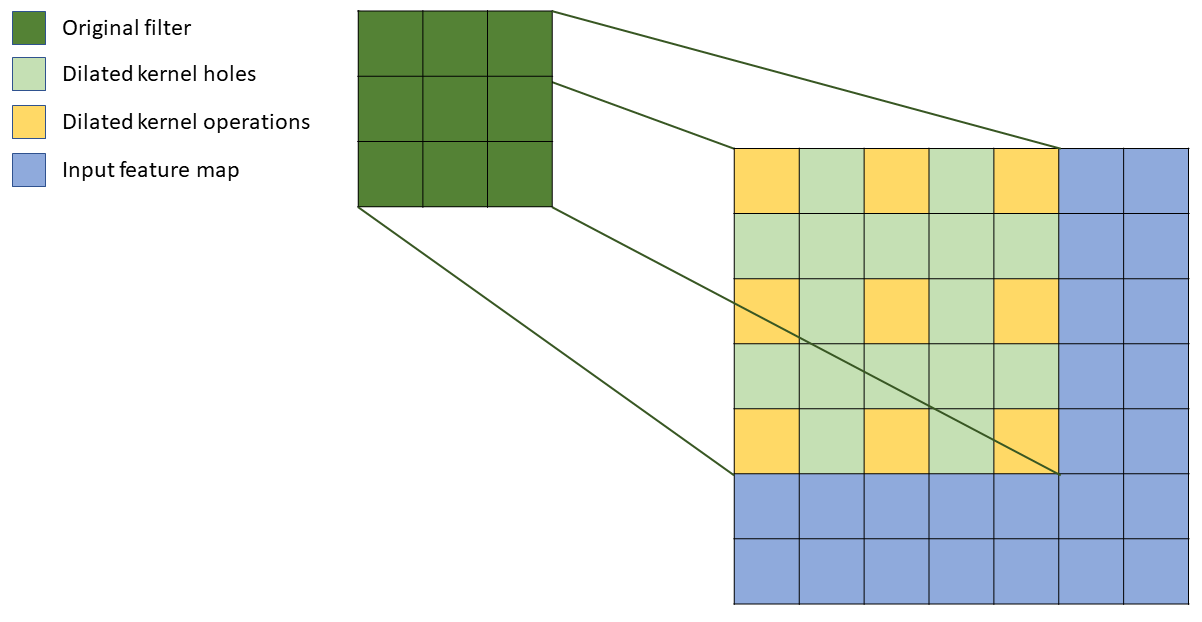
\includegraphics[width=0.8\columnwidth]{.//Figure/Sequential/dilated_convolution.png}}
 \caption{Two-dimensional dilated convolution.}
 \label{fig:dilated_convolution}
\end{figure}

\begin{figure}[H]
 \centerline{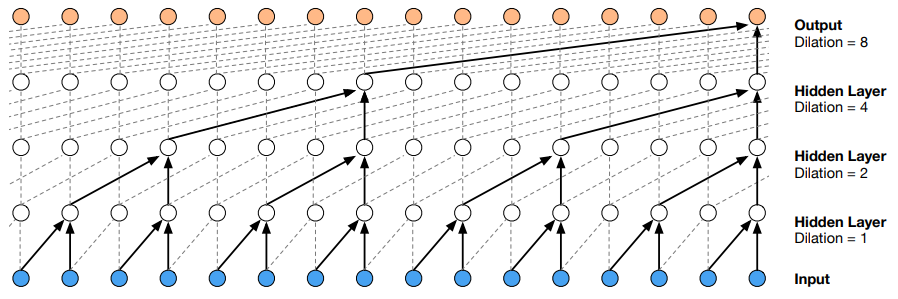
\includegraphics[width=1.0\columnwidth]{.//Figure/Sequential/WaveNet_dilation.png}}
 \caption{Stack of one-dimensional dilated convolutional layers in WaveNet. Source: \cite{WaveNet}}
 \label{fig:WaveNet_dilation}
\end{figure}

These models use solely convolutional layers, thus being relatively simple. While training, the simple backpropagation algorithm is used, and their runtime is fast. However, these models lack one crucial element to process long sequential inputs: memory.

\section{Recurrent neural networks}

Classical neural networks are directed acyclic graphs (DAG), which define computational nodes and their connections. \textit{Recurrent neural networks} (RNN) are dynamic models containing recurrent links (directed loops). These connections can model an inner/hidden state (memory), which makes them useful when sequential data is processed, where later values depend on earlier ones. In every time step, the same function is called, meaning that the RNN's nodes and weights are the same. Figure \ref{fig:RNN} represents the inference steps of an RNN. These models do not require prior knowledge of the input data, and they are generally robust to noise\cite{CTC}. The section below discusses how such a network is trained.

\begin{figure}[htb]
 \centerline{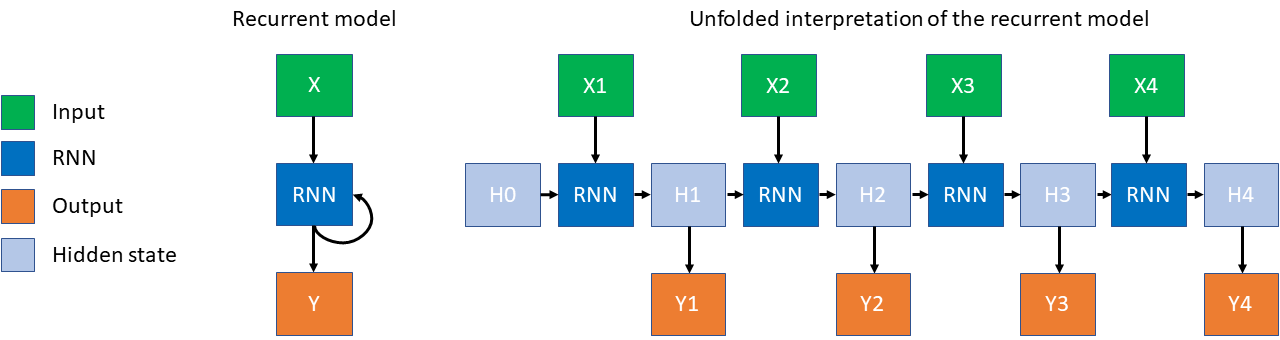
\includegraphics[width=1.0\columnwidth]{.//Figure/Sequential/RNN.png}}
 \caption{Unfolded interpretation of the RNN for a length-4 sequential input.}
 \label{fig:RNN}
\end{figure}

\subsection{Backpropagation through time}

In the classical backpropagation, a model input is first propagated forward the network, resulting in a prediction. When training the network, it is known what is expected from the model's output (ground truth). The difference between the prediction and the ground truth is calculated by the loss function, which results in the network's error. The error is then propagated backward the network: for each connection, a gradient is calculated based on how much it contributed to the local error of the following node. When each link has this value, the algorithm updates each connection weight based on its gradient and the learning rate.

Backpropagation through time\cite{SequentialLecture} (BPTT) works similarly. The difference is that the RNN is handled as an unfolded model. For each time step, the backpropagation algorithm is applied in a manner that the input of the \textit{Nth} step is the output of the \textit{N-1th} step (this wording is intentional, as we are moving backward in time). Gradient values are calculated for the whole network independently for each time step. When gradients are computed for a step, values are updated for each weight (Figure \ref{fig:BPTT}).

\begin{figure}[htb]
 \centerline{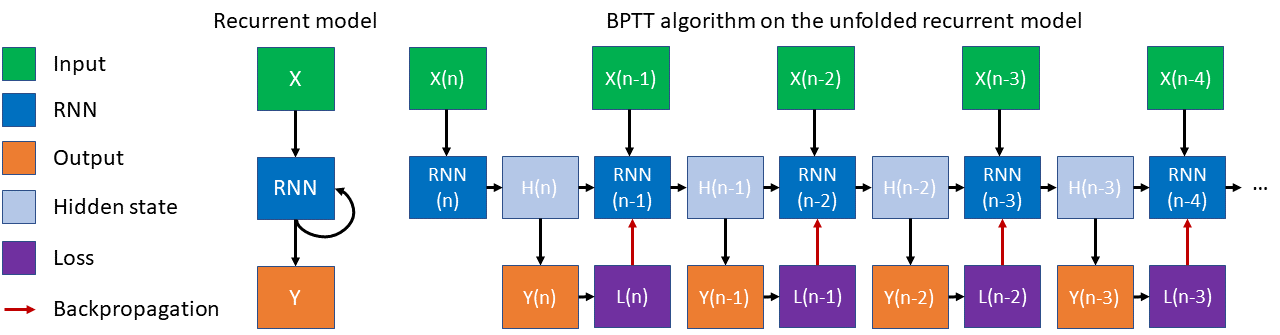
\includegraphics[width=1.0\columnwidth]{.//Figure/Sequential/BPTT.png}}
 \caption{Operation of the BPTT algorithm on the unfolded RNN.}
 \label{fig:BPTT}
\end{figure}

Usually, there is a truncation in the BPTT algorithm: the backward calculation only goes back to the last \textit{K} steps on the network unfolded by time. Otherwise, in the case of long series, the algorithm would take a lot of computational resources, significantly slowing down the training process.

\subsection{Limitations}

Many time steps are needed to create long-term inner memory. During BPTT, the error propagates back to these time steps on the same model. It means that we multiply the model's weight matrix multiple times, which is prone to the following problems:

\begin{itemize}
\item When the weight matrix singular value is high, it leads to gradient exploding. The weight updates are too big, so the model cannot converge.
\item When the weight matrix singular value is low, gradient vanishing happens. In this case, the gradients are too close to zero; weight updates are too small to improve the model.
\end{itemize}

For gradient exploding, possible solutions can be using saturating nonlinear activation functions or gradient clipping, where the values cannot go above a maximum. Skip connections can somehow compensate for the gradient vanishing problem, through which the error can flow freely back to the earlier time steps. However, these are not complete solutions.

\section{Long short-term memory}

Long short-term memory\cite{LSTM} (LSTM) is a type of RNN cell which uses a gated approach. It implements a short-term memory that can be long enough to handle longer sequences than simple RNNs can do. An LSTM cell has three inputs in each time step:

\begin{itemize}
\item \textit{C}: The cell state is the interpretable, optimized output of the cell.
\item \textit{H}: Hidden state, which is the inner state of the LSTM block.
\item \textit{X}: Input tensor, the input from the earlier network layers (for example, a feature map created by convolutional layers which we want to process sequentially, from left to right).
\end{itemize}

There are multiple trainable gates within an LSTM cell, manipulating the signal flow and thus modeling what information is needed from a specific input given a state. These gates are trainable to model memory. The gates are the following:

\begin{itemize}
\item \textit{forget}: Responsible for deleting certain things from the cell state based on the fused input of the hidden state and the input tensor. This gate was not part of the initial publication; it was added a few years later\cite{LSTM-ForgetGate}. Forget gate allows the cell to reset its state and was crucial to the success of LSTM.
\item \textit{input}: Decides what items of the fused input should be written to the cleaned cell state.
\item \textit{gate}: Applies nonlinearity to the fused input written to the cell state. This is the only gate that uses the tanh activation function instead of the sigmoid. This gate projects the values between [-1, 1] to provide the necessary abstraction switching of the signal while maximizing the output range, retaining the saturating behavior. The other gates use sigmoid activation because they mask the signal to be retained (where the minimum is 0 and the maximum is 1).
\item \textit{output}: Masks the hidden state output derived from the cell state.
\end{itemize}

In an LSTM cell, there are only saturating nonlinear activation functions, which can handle the gradient exploding problem. There is no activation function between the input- and the output cell state, only one multiplication (forget gate) and one addition. This means that the input signal can propagate to the output without severe decrease, and thus the gradients can backpropagate without downscaling. This path forms a gradient highway across the unfolded model (containing the same LSTM cell of each time step) during BPTT training. This path is essential in solving the gradient vanishing problem induced by the numerous time steps. The visual representation of an LSTM cell is illustrated by Figure \ref{fig:LSTM}.

\begin{figure}[htb]
 \centerline{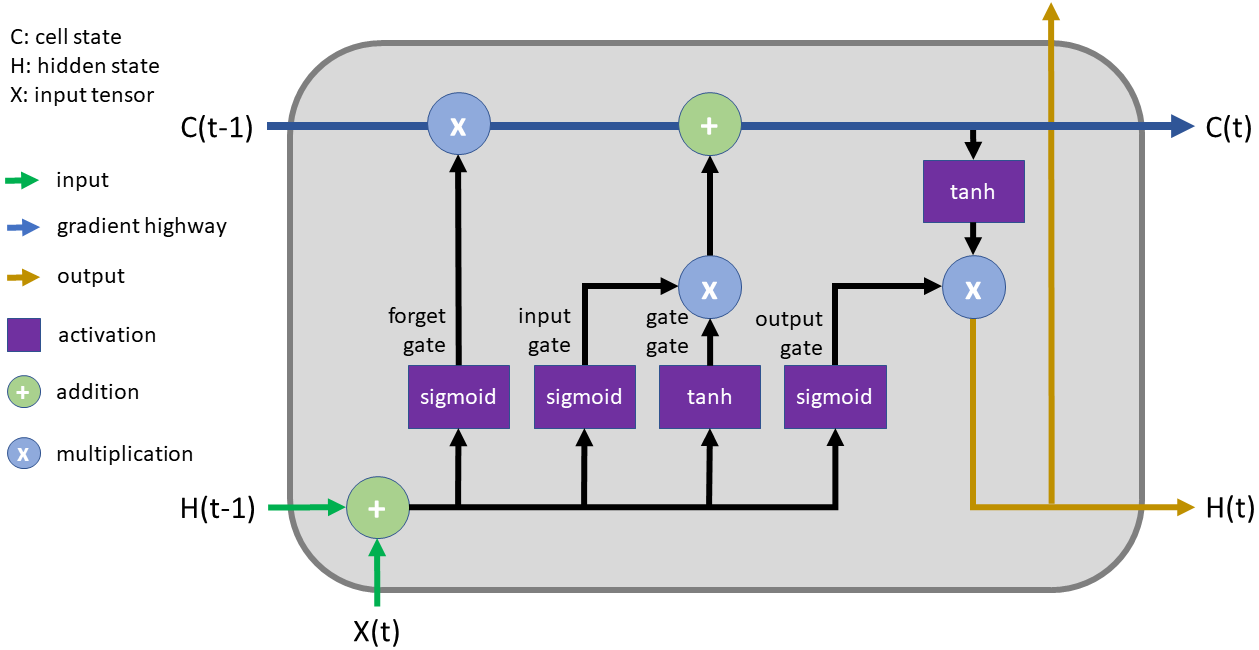
\includegraphics[width=1.0\columnwidth]{.//Figure/Sequential/LSTM.png}}
 \caption{Inner structure of an LSTM cell.}
 \label{fig:LSTM}
\end{figure}

LSTM is a relatively old approach from 1997, a mature standard tool for solving sequential problems. Over time, other solutions have emerged, such as the Gated Recurrent Unit\cite{GRU} (GRU) from 2014, which similarly models memory, but with fewer parameters (three gates instead of four). I decided to present LSTM because it is easier to understand thanks to its well-separated elements.

\section{Connectionist Temporal Classification}

RNNs are good at sequence learning, but they require thoroughly segmented and labeled data, which is time-consuming. Traditional loss functions like mean squared error cannot work well without properly segmented data because they assume that each item in the sequence is independent. This leads to limited model applicability.

Connectionist Temporal Classification\cite{CTC} is a loss function to handle sequential input, which is noisy and unsegmented. It assumes that the network output is a conditional probability distribution over the label sequences. This way, the loss function transforms the sequential problem into classification, where the model needs to select the most probable label for a given input sequence. 

\subsection{Example}

I illustrate the function's applicability on an example with an input image in which we want to read a text. This example is partly based on \cite{CTCexp}. Reading the text in the image can be modeled as a sequential problem, where we want to process the picture from left to right. Only the input and the ground truth text label are needed when training with CTC. We discard the information where the particular characters are. CTC tries the possible alignments of the ground truth label in the image and sums all the scores. This way, it does not matter where the text is in the picture - the algorithm could find a suitable label alignment when the match value is high. This value should be maximized to the alignments outputting the ground truth label.

Because CTC tries to find the optimal label alignment, a good character encoding is needed to help distinguish good and bad ones. The characters are separated by a blank token (marked as ``|''), which separates the letters. This way, when a wide character is processed and triggers multiple predictions next to each other, we can merge them between the blank tokens to identify the actual letter. This also solves the problem of segregating the same characters next to each other. The encoding approach makes it possible to represent the same text multiple ways, allowing different alignments to match. The neural network is trained to predict the output in this encoded format.

\begin{itemize}
\item The word ``curent'' is recognized when the output is ``||ccu|rre|nn|t'', ``|ccc|uu|rr|eee|nnn|ttt|'', or ``c|u|r|e|n|t''.
\item The word ``current'' is recognized when the output is ``||cc||u|rr|renn|t'', ``|ccccuu|rr|rrrreeennn|ttt|'', or ``c|u|r|r|e|n|t''.
\end{itemize}

To calculate the scores for an alignment, we have to consider all the possible paths and sum the ones producing the same decoded text. The added up probability is the overall score of the path. Each path text is then compared to the ground truth label, and the loss value is calculated weighted by the path probabilities. The loss function needs to be minimized. For that, CTC uses the negative sum of the log probabilities. The probability is maximized when this loss is minimized, so the function motivates the model to find good predictions.

The model outputs a matrix containing a score for each character at each time step. There are different approaches to decode this matrix. One method is called \textit{best path decoding}, where:

\begin{itemize}
\item The algorithm takes the maximum prediction at each step, producing the most probable path.
\item To decode the prediction, the same characters are removed next to each other, then the blank tokens are also removed. The remaining output is the predicted text.
\end{itemize}

This method is fast and usually good, but it is just an approximation. There are different decoding approaches where multiple paths can be considered (similarly when calculating the CTC loss for the different paths). One other algorithm is Word Beam Search\cite{WordBeamSearch}, where the number of nodes to consider at each time step can be defined. It can make decoding more accurate but also scalable.